\documentclass[12pt,english]{article}
\usepackage[a4paper,bindingoffset=0.2in,%
            left=1in,right=1in,top=1in,bottom=1in,%
                        footskip=.25in]{geometry}

\usepackage{graphicx} % Required to insert images
\usepackage{amsmath}

\newcommand{\hmwkTitle}{PCA Assignment} % Assignment title
\newcommand{\hmwkClass}{MATH-578} % Course/class
\newcommand{\hmwkClassTime}{} % Class/lecture time
\newcommand{\hmwkAuthorName}{Saket Choudhary} % Your name
\newcommand{\hmwkAuthorID}{2170058637} % Teacher/lecturer
%----------------------------------------------------------------------------------------
%       TITLE PAGE
%----------------------------------------------------------------------------------------

\title{
\vspace{2in}
\textmd{\textbf{\hmwkClass:\ \hmwkTitle}}\\
}

\author{\textbf{\hmwkAuthorName} \\
        \textbf{\hmwkAuthorID}
        }
\date{} % Insert date here if you want it to appear below your name

\begin{document}

\maketitle
\newpage

\section{Part a}

\subsection{Photo Image}
\begin{figure}
%\begin{minipage}{0.5\linewidth}
    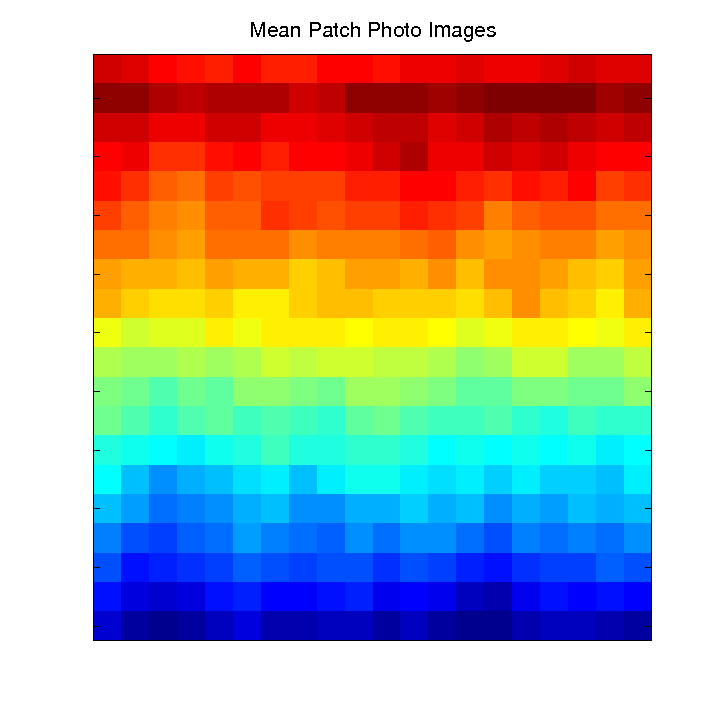
\includegraphics[width=\linewidth]{Mean-Patch-Photo-Images}
    \caption{Mean Patch for Photo Images}
\end{figure}
General feature of Photo Image: Band of colors with gradual descent(colors merge into one another), indicating image has less features(less variance)
overall.
%\end{minipage}
%\begin{minipage}{0.5\linewidth}
\subsection{VTEC Image}
\begin{figure}
    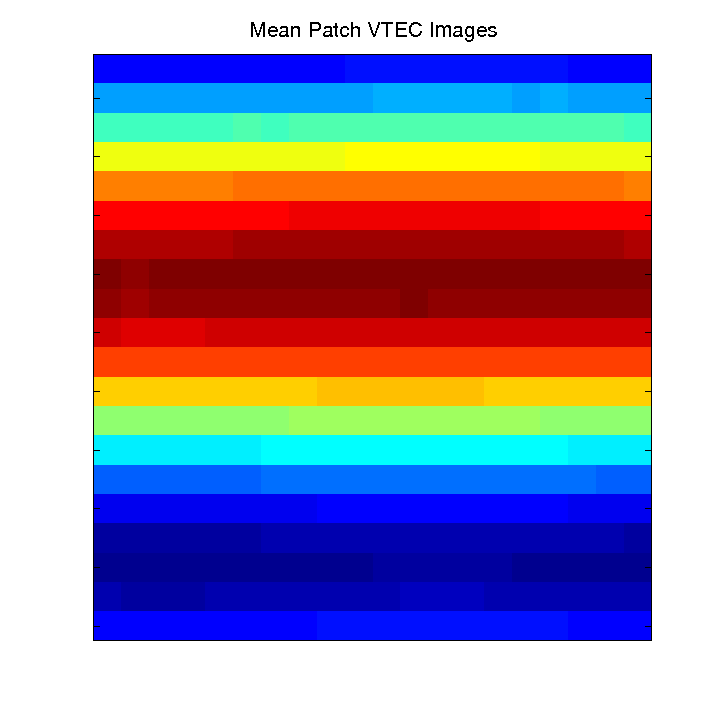
\includegraphics[width=\linewidth]{Mean-Patch-VTEC-Images}
    \caption{Mean Patch for VTEC Images}
%\end{minipage}
\end{figure}

General features of VTEC Image: Band of colors which form a steep gradient(different colors do not merge into one another), indicating
that the image has more features (the total variance is high)

\pagebreak
\newpage
\clearpage

\section{Part b}

\subsection{Photo Image}
\begin{figure}
    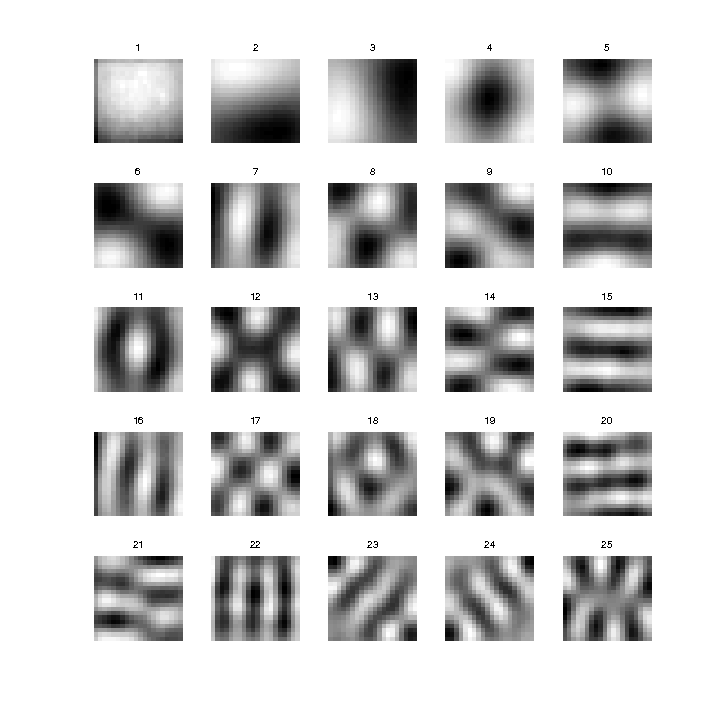
\includegraphics[width=\linewidth]{first25-Photo-Images.png}
    \caption{First 25 eigen vectors of Photo Image. The images exhibit high variance}
\end{figure}

\begin{figure}
    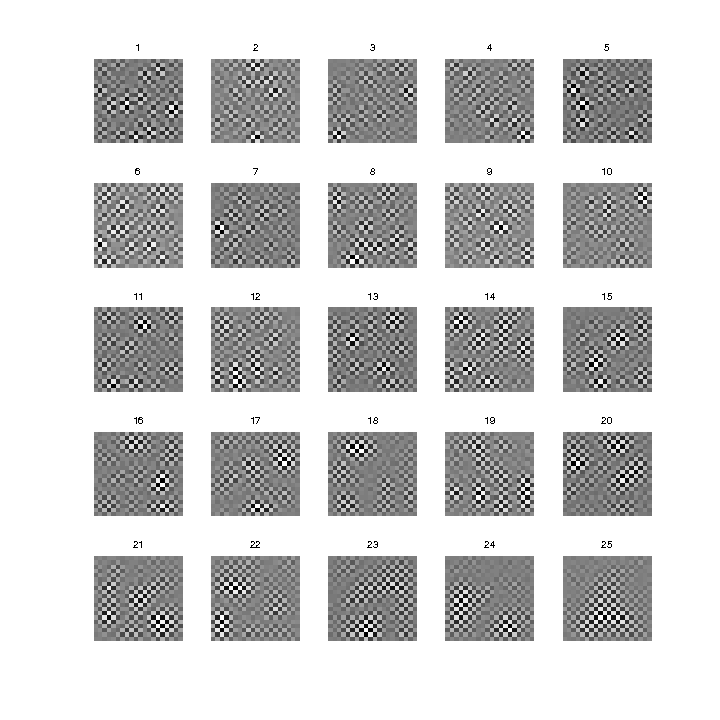
\includegraphics[width=\linewidth]{last25-Photo-Images.png}
    \caption{Last 25 eigen vectors of Photo Image. Images exhibit low variance and hence are indistinguishable}
\end{figure}

\subsection{VTEC Image}
\begin{figure}
    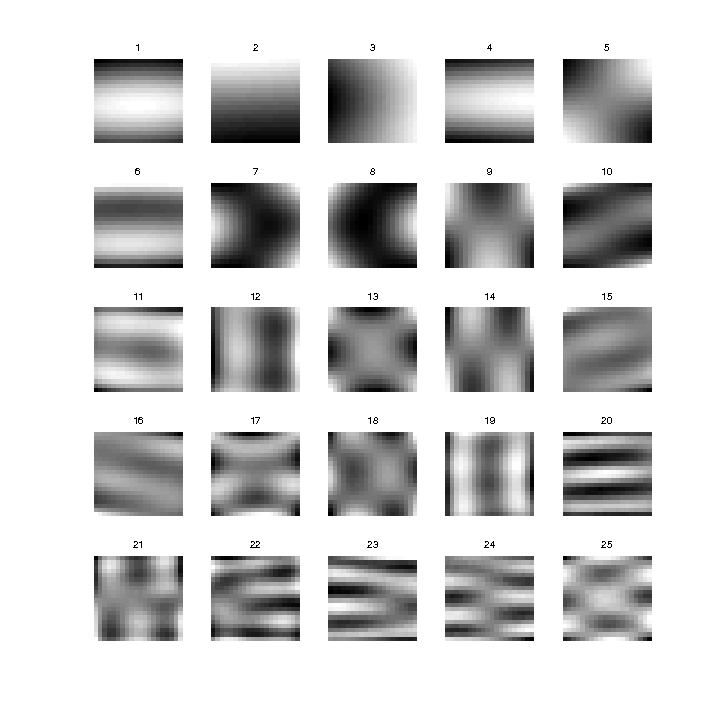
\includegraphics[width=\linewidth]{first25-VTEC-Images.png}
    \caption{First 25 eigen vectors of VTEC Image. Images exhibit high variance.}
\end{figure}

\begin{figure}
    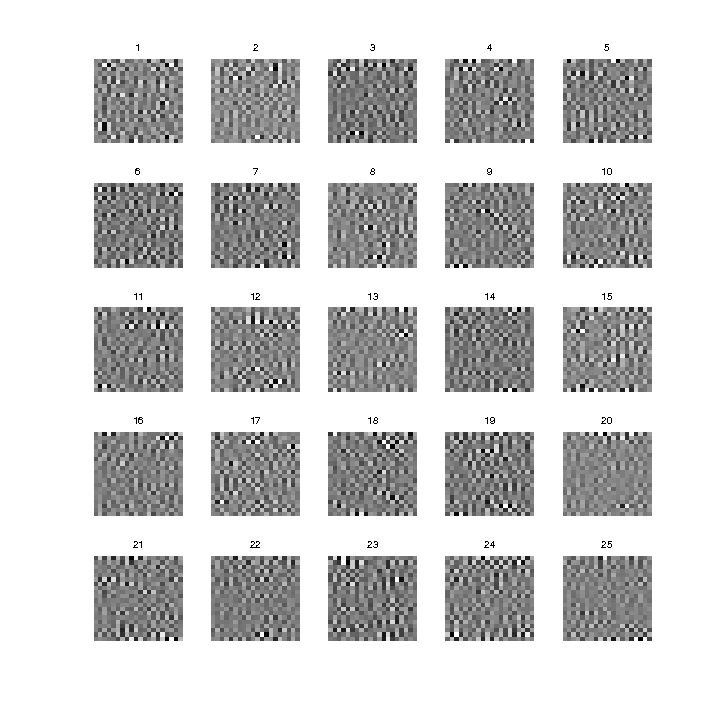
\includegraphics[width=\linewidth]{last25-VTEC-Images.png}
    \caption{Last 25 eigen vectors of VTEC Image. Images exhibit low variance and are indisinguishable} 
\end{figure}

\newpage
\section{Part c,d,e}

Given that we are compressing a $600\times 600$ to a $400\times r$ matrix of eigen vectors(assume the eigen values vetor of length $r$ occupies egligible 
space),
we can simply store this eigen vector matrix, we attain a $\frac{400}{r}\%$ reduction.
For example with $r=1$ we are attaining a $400\%$ reduction, with $r=80$ it is $5\%$.
With $r=10$, it is $40\%$.

\subsection{ Photo Images }
\begin{figure}
\begin{minipage}{0.5\linewidth}
    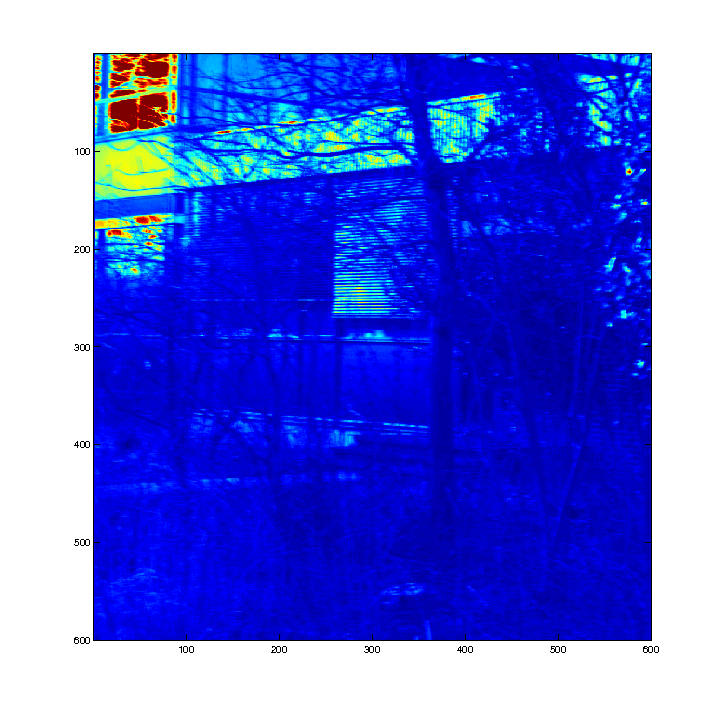
\includegraphics[width=\linewidth]{pca-part-c-Photo_Images-original.png}
    \caption{\footnotesize{Original 170th Photo Image}}
\end{minipage}
\begin{minipage}{0.5\linewidth}
    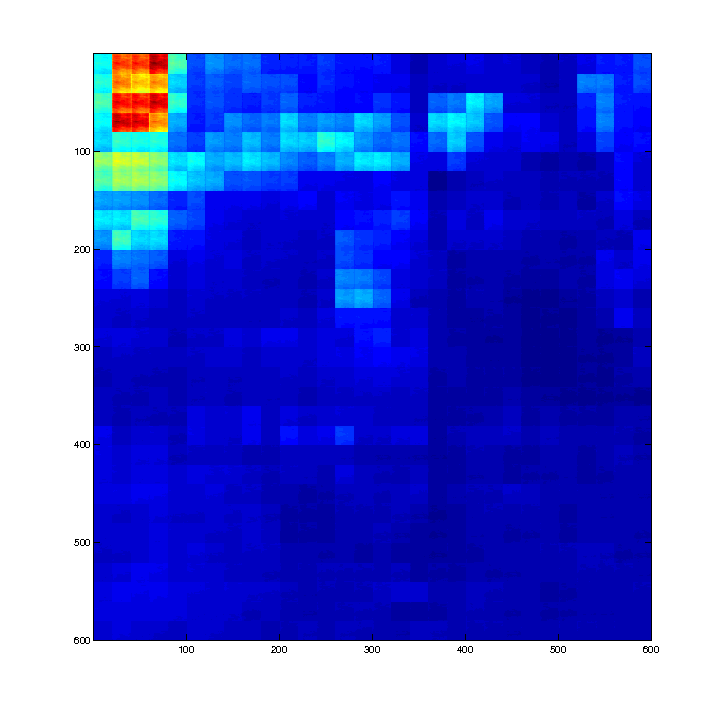
\includegraphics[width=\linewidth]{pca-part-c-Photo_Images-reconstructed-r=1.png}
    \caption{\footnotesize{r=1. \% variance = $78.7749$}}
\end{minipage}
\end{figure}

\begin{figure}
\begin{minipage}{0.5\linewidth}
    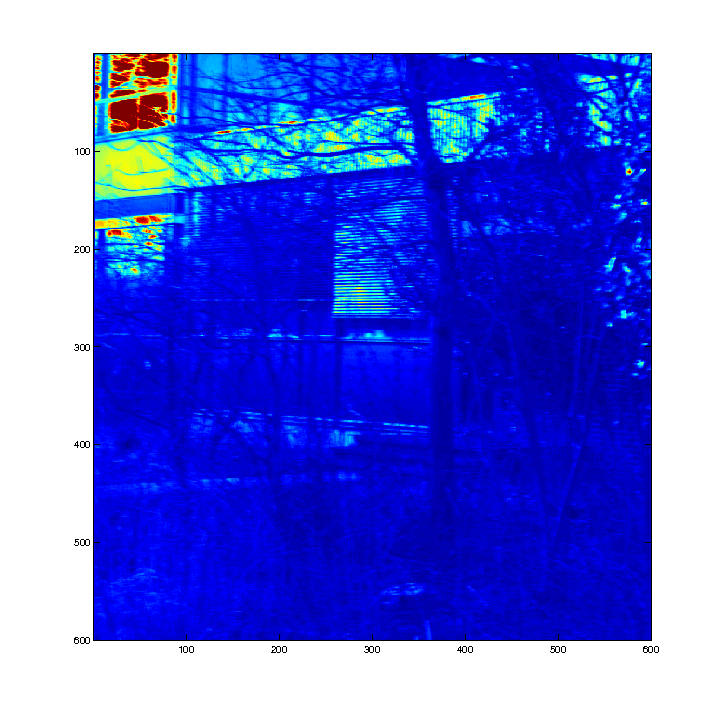
\includegraphics[width=\linewidth]{pca-part-c-Photo_Images-original.png}
    \caption{Original 170th Photo Image}
\end{minipage}
\begin{minipage}{0.5\linewidth}
    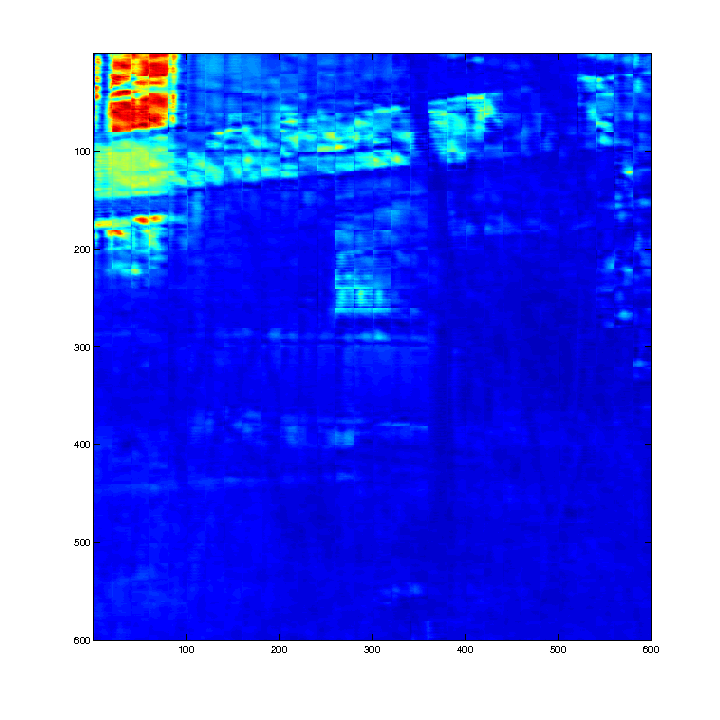
\includegraphics[width=\linewidth]{pca-part-c-Photo_Images-reconstructed-r=10.png}
    \caption{r=10. \% variance = $92.1408$}
\end{minipage}
\end{figure}

\begin{figure}
\begin{minipage}{0.5\linewidth}
    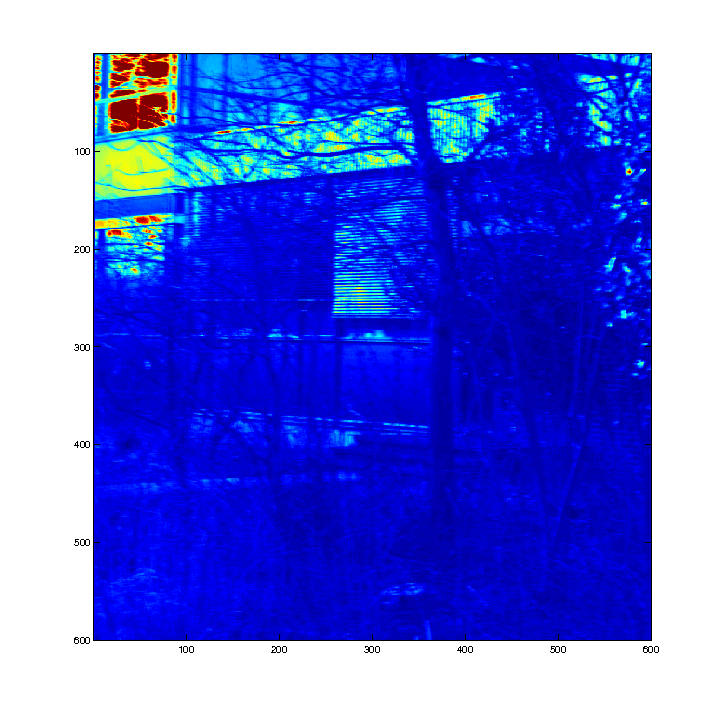
\includegraphics[width=\linewidth]{pca-part-c-Photo_Images-original.png}
    \caption{Original 170th Photo Image}
\end{minipage}
\begin{minipage}{0.5\linewidth}
    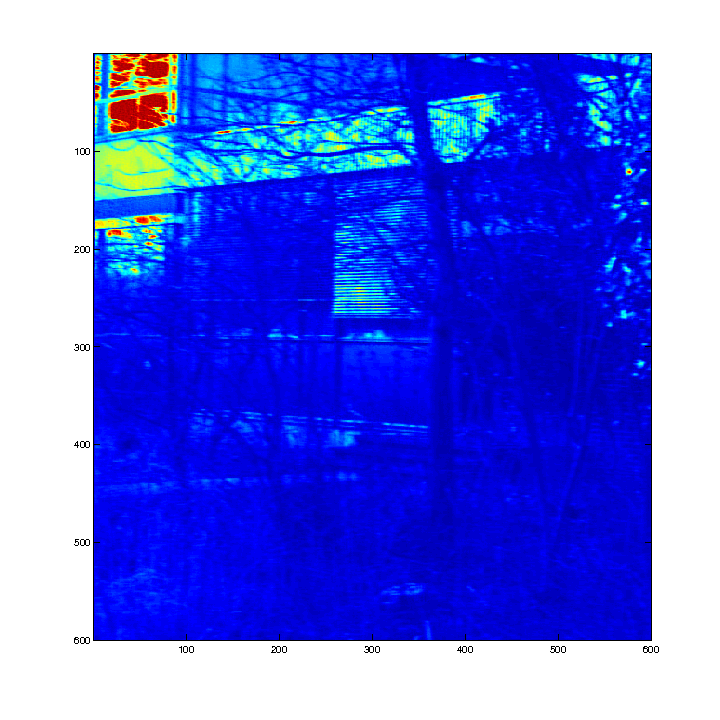
\includegraphics[width=\linewidth]{pca-part-c-Photo_Images-reconstructed-r=80.png}
    \caption{r=80. \% variance = $99.3984$}
\end{minipage}
\end{figure}


\subsection{ VTEC Images }
\begin{figure}
\begin{minipage}{0.5\linewidth}
    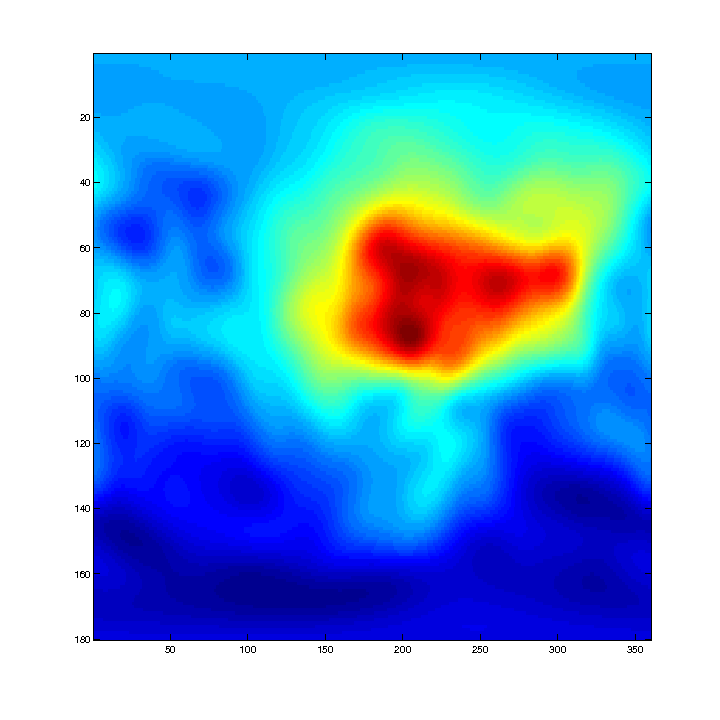
\includegraphics[width=\linewidth]{pca-part-c-VTEC_Images-original.png}
    \caption{\footnotesize{Original 170th VTEC Image}}
\end{minipage}
\begin{minipage}{0.5\linewidth}
    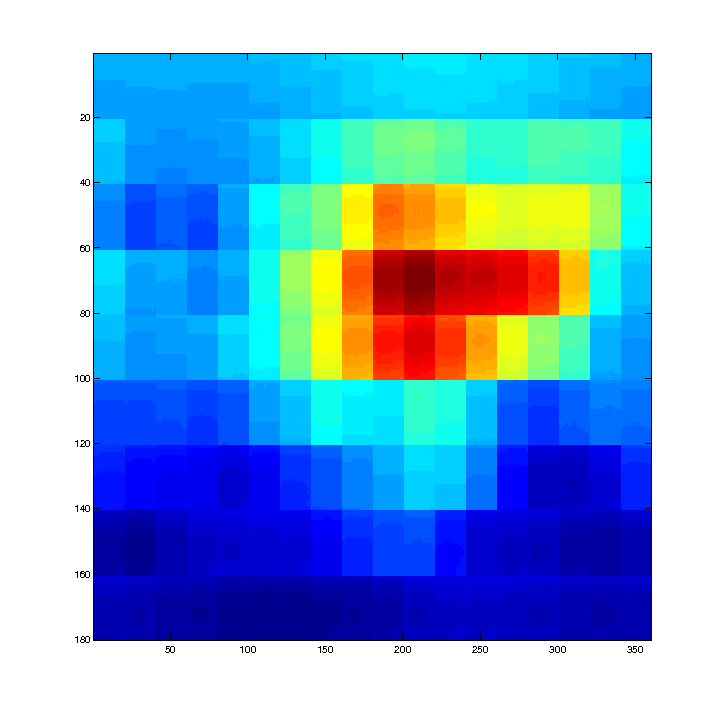
\includegraphics[width=\linewidth]{pca-part-c-VTEC_Images-reconstructed-r=1.png}
    \caption{\footnotesize{r=1. \% variance = $95.3856$}}
\end{minipage}
\end{figure}

\begin{figure}
\begin{minipage}{0.5\linewidth}
    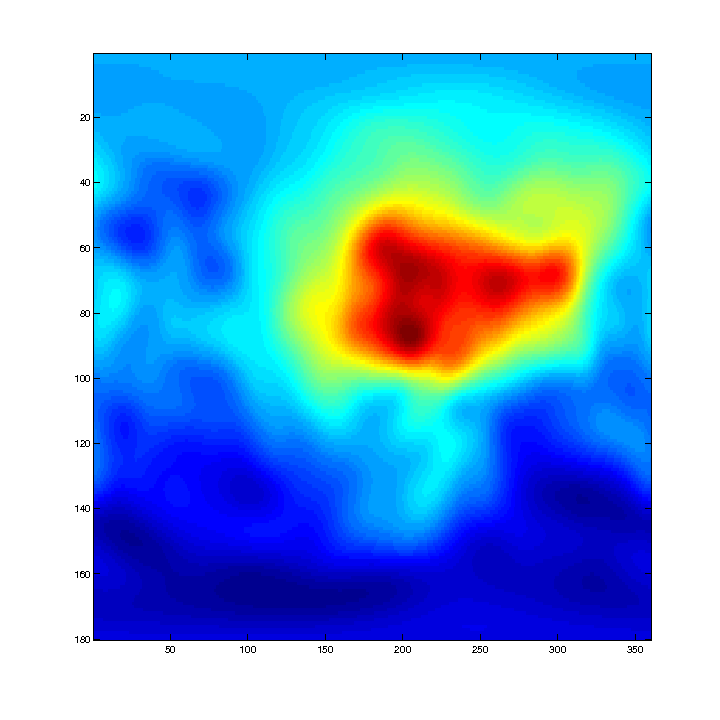
\includegraphics[width=\linewidth]{pca-part-c-VTEC_Images-original.png}
    \caption{Original 170th VTEC Image}
\end{minipage}
\begin{minipage}{0.5\linewidth}
    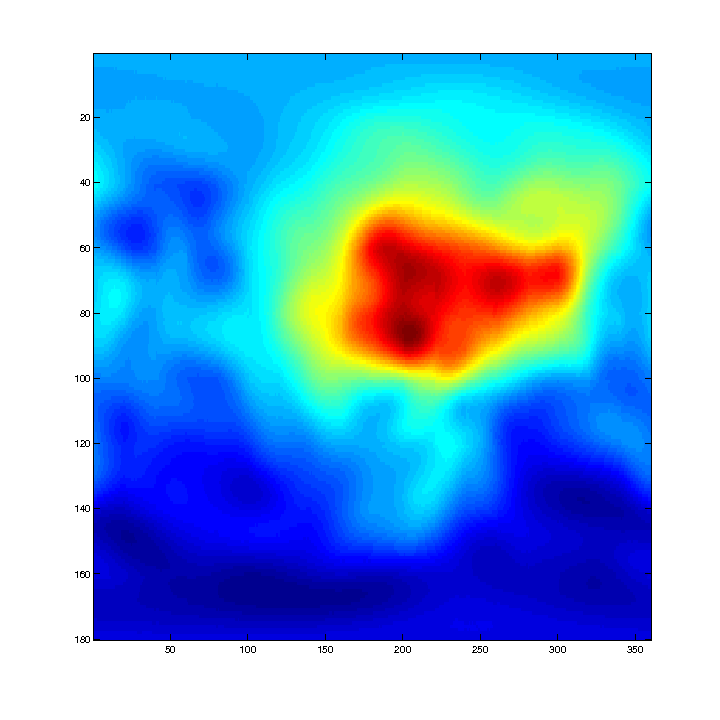
\includegraphics[width=\linewidth]{pca-part-c-VTEC_Images-reconstructed-r=10.png}
    \caption{r=10. \% variance = $99.9930$}
\end{minipage}
\end{figure}

\begin{figure}
\begin{minipage}{0.5\linewidth}
    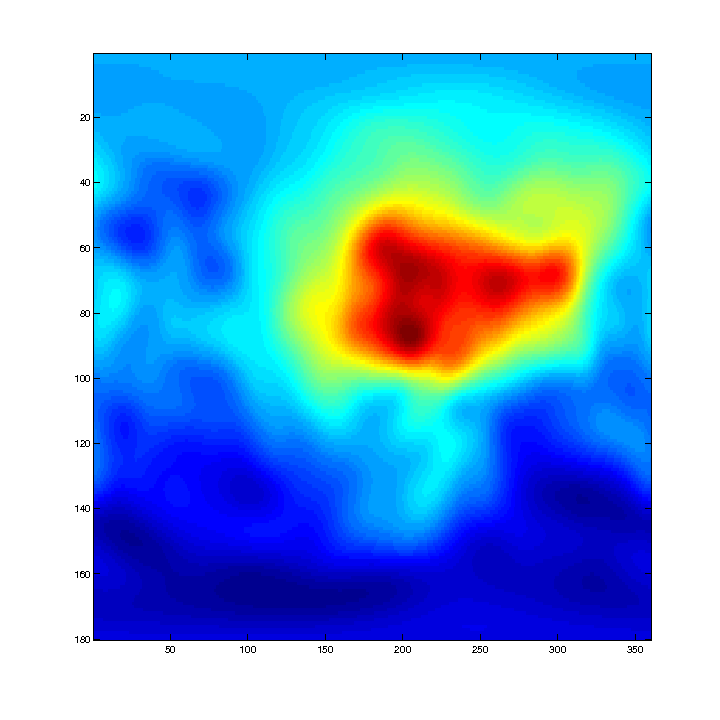
\includegraphics[width=\linewidth]{pca-part-c-VTEC_Images-original.png}
    \caption{Original 170th VTEC Image}
\end{minipage}
\begin{minipage}{0.5\linewidth}
    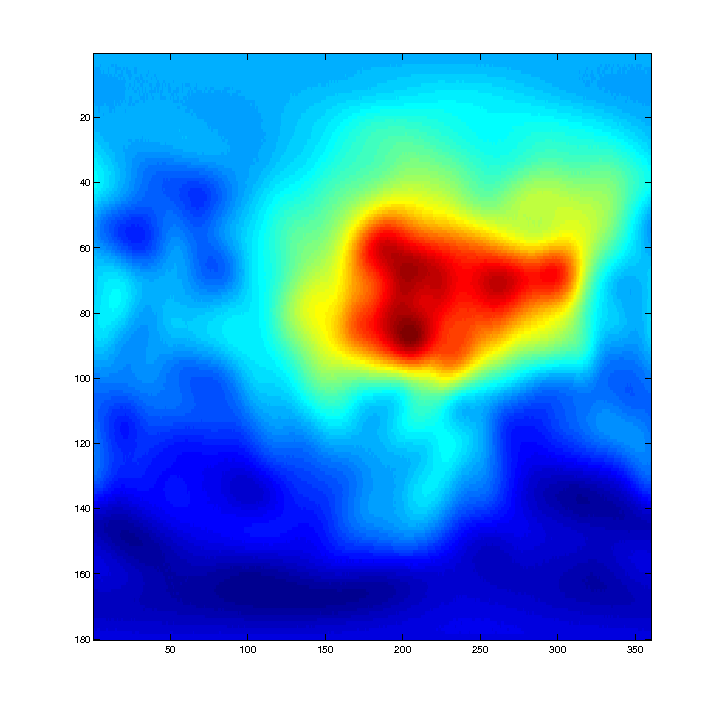
\includegraphics[width=\linewidth]{pca-part-c-VTEC_Images-reconstructed-r=80.png}
    \caption{r=80. \% variance = $99.9991$}
\end{minipage}
\end{figure}


\end{document}
